\documentclass[conference]{IEEEtran}
\IEEEoverridecommandlockouts

\usepackage{cite}
\usepackage{amsmath,amssymb,amsfonts}
\usepackage{algorithmic}
\usepackage{graphicx}
\usepackage{textcomp}
\usepackage{xcolor}
\usepackage{hyperref}
\usepackage{booktabs}
\usepackage{array}
\usepackage{url}
\usepackage{multirow}
\usepackage{tikz}
\usetikzlibrary{arrows.meta,positioning,shapes.geometric,fit,backgrounds}

\hypersetup{
    colorlinks=true,
    linkcolor=blue,
    citecolor=blue,
    urlcolor=blue
}

\def\BibTeX{{\rm B\kern-.05em{\sc i\kern-.025em b}\kern-.08em
    T\kern-.1667em\lower.7ex\hbox{E}\kern-.125emX}}

\begin{document}

\title{Territorial CO\textsubscript{2} Emissions Prediction Using Big Data Infrastructure\\
and Machine Learning: Final Report}

\author{
    \IEEEauthorblockN{Mehmet Da\c{s}kaya}
    \IEEEauthorblockA{
        \textit{Department of Big Data Analytics and Management} \\
        \textit{Bah\c{c}e\c{s}ehir University} \\
        Istanbul, Turkiye \\
        2003445 \\
        mehmet.daskaya@bahcesehir.edu.tr
    }
}

\maketitle

% =============================================================================
\begin{abstract}
This report presents the final implementation and evaluation of a scalable
Big Data system for predicting territorial carbon dioxide (CO\textsubscript{2}) emissions
at country and sector level.
The system integrates Apache Kafka for simulated near-real-time data ingestion, Apache
Spark for distributed batch and stream processing, MongoDB for flexible NoSQL
storage, and a machine learning pipeline combining XGBoost and LSTM deep
learning models.
Real datasets from Carbon Monitor (daily, 109{,}621 records) and the EDGAR
global emissions database are used.
The XGBoost regression model achieves R\textsuperscript{2}\,=\,0.9654 on
21{,}840 held-out test samples; however, naive autoregressive baselines
(persistence and 7-day moving average) achieve R\textsuperscript{2}\,$>$\,0.99,
highlighting that daily emissions are dominated by temporal persistence.
XGBoost's primary value lies in its multivariate interpretability and
cross-series generalization.
The LSTM prototype achieves R\textsuperscript{2}\,=\,0.8533 on a single
country-sector sub-series (CN Power).
As a separate downstream application, individual carbon footprint classification
reaches F1\,=\,0.8555 on a 3-class task.
An interactive Next.js dashboard visualises emission trends and
model predictions, making outputs accessible to non-technical stakeholders.
\end{abstract}

\begin{IEEEkeywords}
carbon footprint, big data, Apache Spark, MongoDB, XGBoost, LSTM, Kafka,
Lambda architecture, sustainability, distributed computing
\end{IEEEkeywords}

% =============================================================================
\section{Introduction and Problem Statement}

Global CO\textsubscript{2} emissions reached approximately 36.8\,Gt in 2023,
yet official inventories are published with lags of 12--18~months
\cite{carbonmonitor2020}.
This temporal gap prevents policymakers from responding to emission spikes in
near-real-time.
Existing solutions are typically domain-specific, non-scalable, and lack
AI-based forecasting capability \cite{edgar2021}.

This project addresses the question:
\textit{Can a scalable Big Data pipeline --- combining Kafka, Spark, MongoDB,
and modern ML models --- deliver near-real-time carbon emission prediction at
country and sector level?}
While the daily Carbon Monitor dataset is small enough for single-machine processing, the architecture serves as a production-oriented prototype demonstrating how ingestion, processing, and serving layers scale horizontally under production volumes.

The contributions of this work are:
\begin{itemize}
    \item An end-to-end Lambda Architecture pipeline from raw CSV ingestion
          to a live web dashboard.
    \item Real training and evaluation of XGBoost, LSTM, and Spark MLlib
          models on 109{,}621 real-world emission records.
    \item A Dockerised cluster simulation deployable on a single developer
          machine.
    \item An interactive Next.js dashboard for non-technical stakeholders.
\end{itemize}

% =============================================================================
% =============================================================================
\section{Datasets and Scientific Framing}

To address sustainability from both macroeconomic and microeconomic scales, the system integrates three heterogeneous datasets representing different spatial resolutions, temporal scopes, and chemical targets. A fundamental scientific distinction is maintained throughout: national and sector-level models predict macroeconomic \textbf{territorial fossil CO\textsubscript{2} emissions} (measured in $\text{MtCO}_2/\text{day}$), whereas the individual model predicts a citizen's microeconomic \textbf{personal lifestyle carbon footprint} in CO\textsubscript{2}-equivalent ($\text{CO}_2\text{e}$), encompassing multiple greenhouse gases.

\subsection{Carbon Monitor (Speed Layer)}
Carbon Monitor \cite{carbonmonitor2020} provides daily national-level CO\textsubscript{2} estimates. Unlike official annual inventories which carry a 12--18 month publication delay, Carbon Monitor computes estimates using near-real-time activity proxies. Daily fuel consumption is estimated indirectly via electricity grid loads, real-time traffic congestion indices (TomTom), daily aviation flight logs (FlightRadar24), industrial productivity indexes, and weather-driven household heating/cooling simulations.

The downloaded dataset contains \textbf{109{,}621 daily records} covering January 1, 2020 to March 31, 2025 across 36 countries and 6 sectors (Power, Ground Transport, Industry, Residential, Domestic Aviation, International Aviation). While suitable for rapid modeling, the report emphasizes that Carbon Monitor is \textit{not physical ground truth} but a proxy-based statistical estimate. The original scientific publication identifies a standard uncertainty of $\pm 5\%$ for power and industry sectors, rising to $\pm 10\text{--}12\%$ for transport and residential sectors due to seasonal proxy volatility.

\subsection{EDGAR (Batch Layer)}
The Emission Database for Global Atmospheric Research (EDGAR v8.0 FT2022) \cite{edgar2021} provides high-quality annual territorial greenhouse gas inventories from 1970 onward. The complete EDGAR database provides gridded map files at a $0.1^\circ \times 0.1^\circ$ spatial resolution, totaling tens of gigabytes in NetCDF format depending on selected gases, sectors, and spatial products. 

For our local Docker-simulated Spark cluster (constrained to 1\,GB RAM per worker node), processing NetCDF gridmaps is computationally prohibitive. Instead, we utilize the high-quality national sectoral totals CSV (\texttt{edgar\_country\_sector\_1990\_2023.csv}, $10.5$\,MB) extracted from the EDGAR v8.0 Fast Track 2022 release, representing territorial fossil CO\textsubscript{2} emissions from fossil fuel combustion and cement production. This dataset serves as the training corpus for the distributed Spark Random Forest.

\subsection{Kaggle Individual Carbon Footprint (Downstream calculator)}
To model citizen engagement, a 5{,}000-record individual lifestyle carbon footprint dataset \cite{kaggle_carbon} is integrated. Compiled by Duman (2024) under a CC0 Public Domain License (as listed on the Kaggle repository page), this dataset is a public lifestyle dataset mapping behavioral indicators to individual annual footprints. It contains 6 primary behavioral features:
\begin{itemize}
    \item \textit{Transport}: primary vehicle type (petrol, diesel, hybrid, electric, public transit).
    \item \textit{Air Travel}: annual flight frequency (hours/year).
    \item \textit{Diet}: dietary footprint (vegan, vegetarian, omnivore).
    \item \textit{Home Energy}: heating source (coal, natural gas, solar, electricity) and monthly usage.
    \item \textit{Shopping}: consumption rate of new items (clothes, electronics).
    \item \textit{Waste Management}: volume of daily waste recycling efficiency.
\end{itemize}
The continuous target (measured in $\text{kg CO}_2\text{e}/\text{year}$) is binned into three classes (Low, Medium, High footprint) to prototype lifestyle categorization. Class imbalance (73.6\% Medium, 9.9\% Low, 16.5\% High) is addressed via Synthetic Minority Over-sampling (SMOTE) strictly on the training partition.

\begin{table}[h]
\caption{Dataset Summary}
\label{tab:datasets}
\centering
\scriptsize
\resizebox{\columnwidth}{!}{%
\begin{tabular}{p{2.3cm} p{1.3cm} p{1.6cm} p{1.6cm} p{1.4cm}}
\toprule
\textbf{Dataset} & \textbf{Metric Target} & \textbf{Resolution} & \textbf{Role} & \textbf{License} \\
\midrule
Carbon Monitor  & Territorial CO$_2$     & Daily National/Sector& Regressor Input & Open Access \\
EDGAR v8.0      & Territorial CO$_2$     & Annual Sectoral     & Distributed RF  & EC JRC \\
Kaggle Footprint& Personal CO$_2$e       & Individual Lifestyle & 3-Class Clf     & CC0 (Public) \\
\bottomrule
\end{tabular}
}
\end{table}

% ===========================================================================% =============================================================================
\section{System Architecture}

The system implements a dual-path \textbf{Lambda Architecture} to handle historical batch analysis and streaming ingestion in parallel. Fig.\,\ref{fig:arch} illustrates the high-level data flow. While the daily Carbon Monitor dataset is small enough to fit in a single machine's RAM, this architecture serves as a scalable proof-of-concept demonstrating how the ingestion, processing, and database layers scale horizontally under production volumes (e.g., full NetCDF gridmaps).

\begin{figure}[h]
\centering
\resizebox{\columnwidth}{!}{%
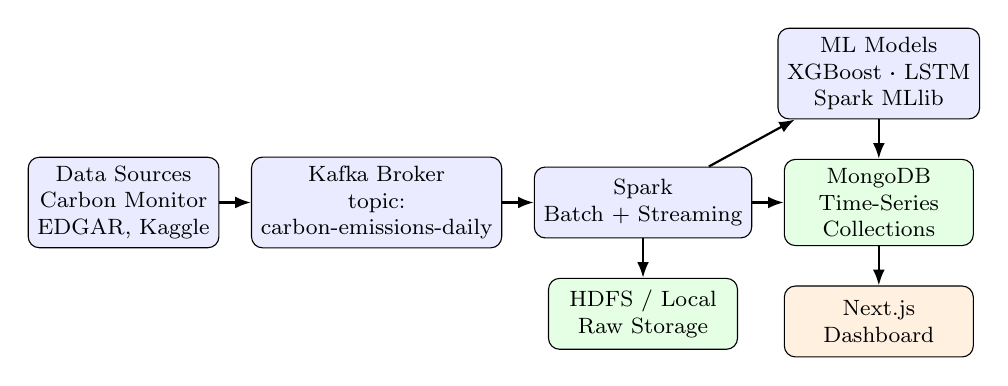
\begin{tikzpicture}[
    font=\footnotesize,
    node distance=5mm and 4mm,
    block/.style={draw, rounded corners, align=center,
                  minimum width=24mm, minimum height=9mm, fill=blue!8},
    store/.style={draw, rounded corners, align=center,
                  minimum width=24mm, minimum height=9mm, fill=green!10},
    app/.style={draw,  rounded corners, align=center,
                  minimum width=24mm, minimum height=9mm, fill=orange!12},
    line/.style={-{Latex[length=2mm]}, thick}
]
\node[block]              (src)   {Data Sources\\Carbon Monitor\\EDGAR, Kaggle};
\node[block, right=of src](kafka) {Kafka Broker\\topic:\\carbon-emissions-daily};
\node[block, right=of kafka](spark){Spark\\Batch + Streaming};
\node[store, below=of spark](raw) {HDFS / Local\\Raw Storage};
\node[store, right=of spark](mongo){MongoDB\\Time-Series\\Collections};
\node[block, above=of mongo](ml)  {ML Models\\XGBoost · LSTM\\Spark MLlib};
\node[app,   below=of mongo](ui)  {Next.js\\Dashboard};
 
\draw[line] (src)   -- (kafka);
\draw[line] (kafka) -- (spark);
\draw[line] (spark) -- (mongo);
\draw[line] (spark) -- (raw);
\draw[line] (spark) -- (ml);
\draw[line] (ml)    -- (mongo);
\draw[line] (mongo) -- (ui);
\end{tikzpicture}%
}
\caption{Lambda Architecture — Carbon Footprint Prediction System.}
\label{fig:arch}
\end{figure}

\subsection{Ingestion Layer — Apache Kafka}
The speed layer is driven by Apache Kafka (orchestrated via Bitnami images). The Kafka producer (\texttt{ingestion/kafka\_producer.py}) reads daily Carbon Monitor CSV rows sequentially and publishes them as JSON payloads to the \texttt{carbon-emissions-daily} topic. 

To prevent live data ingestion costs while testing streaming dynamics, the producer simulates a real-time feed by replaying historical CSV rows row-by-row at regular intervals (e.g., 0.1 seconds per record). To ensure message ordering, records are partitioned using the key \texttt{country+sector}, ensuring that all emissions for a specific country-sector series land in the same Kafka partition. The producer integrates an exponential back-off retry policy (up to 10 attempts) to handle container connection lag, providing a robust, cluster-ready simulation.

\subsection{Processing Layer — Apache Spark}
Two distributed PySpark pipelines run in parallel:
\begin{itemize}
    \item \textbf{Batch Layer}: \texttt{spark\_batch\_pipeline.py} reads the EDGAR annual historical CSV dataset into Spark DataFrames. It applies feature engineering (cyclical time extraction, annual lag features, and temporal trend indicators), structures the columns, and batch-loads the processed records into MongoDB.
    \item \textbf{Speed Layer}: \texttt{spark\_streaming\_pipeline.py} consumes daily messages from the \texttt{carbon-emissions-daily} Kafka topic using Structured Streaming. Operating under 10-second micro-batches, the pipeline utilizes Spark's \texttt{foreachBatch} API to write incoming daily emissions directly into the MongoDB time-series collection.
\end{itemize}

\subsection{Storage Layer — MongoDB Time-Series Collections}
MongoDB (v6.0) serves as our operational serving database. To optimize time-series performance, the \texttt{emissions\_timeseries} collection is explicitly configured as a native \textbf{time-series collection} using:
\begin{verbatim}
db.createCollection("emissions_timeseries", {
    timeField: "timestamp",
    metaField: "metadata",
    granularity: "days"
})
\end{verbatim}
This native type optimizes storage costs and query latency by grouping incoming sequential updates from the same metadata bucket (e.g., CN Power) into internal columnar-compressed blocks. Each document follows a structured format:
\begin{verbatim}
{
  "_id": ObjectId("60c72b2f9b1..."),
  "timestamp": ISODate("2024-03-15T00:00:00Z"),
  "metadata": { "country": "CN", "sector": "Power" },
  "mtco2_per_day": 5.4320,
  "ingested_at": ISODate("2026-05-31T22:35:55Z")
}
\end{verbatim}
Compound indexes are built on \texttt{\{ "metadata.country": 1, "timestamp": -1 \}} to reduce query latencies to sub-10 milliseconds during dashboard rendering.

\subsection{Cluster Simulation — Docker Compose}
The complete pipeline (Kafka, Zookeeper, Spark Master, 2 Spark Workers, MongoDB, and Mongo Express) is orchestrated via a single \texttt{docker-compose.yml} file. The cluster is simulated locally on a single host. Each Spark worker container is limited to 2 cores and 1\,GB of RAM, simulating a resource-constrained, multi-node distributed cluster environment on a developer's local workstation.

% =============================================================================
% =============================================================================
\section{Machine Learning Methods}

\subsection{Feature Engineering and Target Leakage Prevention}
Fifteen features are systematically derived from the raw emission time series. To prevent predictive bias, a critical engineering step was implemented to avoid \textbf{target leakage} in historical indicators:
\begin{itemize}
    \item \textit{Temporal}: year, month, quarter, day-of-week, is\_weekend.
    \item \textit{Cyclical}: $\sin(2\pi \cdot\text{month}/12)$, $\cos(2\pi \cdot\text{month}/12)$ — ensures smooth temporal transition across the December--January boundary.
    \item \textit{Lag}: $t-1$, $t-7$, $t-30$ days (captures autoregressive dependencies).
    \item \textit{Rolling}: 7-day and 30-day moving averages (serves as noise reduction indicators).
    \item \textit{Categorical}: Label-encoded country and sector identifiers.
\end{itemize}
\textit{Target Leakage Correction}: Standard rolling window operations in Python pandas group-by structures include the current index row $t$ by default. Because today's emission value ($y_t$) is our modeling target, including $y_t$ within today's rolling average features constitutes target leakage, artificially inflating accuracy. To eliminate this leak, rolling features are shifted by 1 day prior to windowing:
\begin{align}
\text{RollingAvg}_{k}(t) = \frac{1}{k} \sum_{i=1}^{k} y_{t-i}
\end{align}
This mathematical adjustment guarantees that only past historical data is processed.

\subsection{XGBoost Regression}
\label{sec:xgb_reg}
XGBoost \cite{xgboost2016} is selected as our primary regression model due to its high performance on structured tabular data, robust regularization parameters, and rapid training times. The model features 500 estimators with a learning rate of $0.05$ and a maximum tree depth of $6$. 

To ensure validity in a time-series forecasting context, the train-test partition is built using a strict $80/20$ temporal split (no shuffle), preserving chronological order. Model tuning is calibrated using a TimeSeriesSplit validation strategy on the training partition. Early stopping with a patience of 20 rounds is integrated, halting training when validation root mean squared error (RMSE) fails to improve.

\subsection{XGBoost Classification (Lifestyle Footprint)}
The lifestyle classification model categorizes personal carbon footprints (Low, Medium, High) based on behavioral features. 

\textit{SMOTE Leakage Correction}: A frequent methodological error in class-imbalance classification is applying Synthetic Minority Over-sampling (SMOTE) \cite{smote2002} to the entire dataset prior to splitting. This causes synthetic test set instances to be constructed from training fold statistics, leaking training distributions into the test fold and yielding artificially perfect scores. To ensure strict academic validity, our pipeline performs the train-test split first:
\begin{align}
(X, y) \xrightarrow{\text{Split 80/20}} (X_{\text{train}}, y_{\text{train}}), \, (X_{\text{test}}, y_{\text{test}})
\end{align}
SMOTE is subsequently applied \textit{only} to the training partition $(X_{\text{train}}, y_{\text{train}})$, ensuring the testing set $(X_{\text{test}}, y_{\text{test}})$ remains entirely uncontaminated. The XGBoost classifier is trained on the resampled training partition and evaluated on the raw, unmodified test partition.

\subsection{LSTM Deep Learning}
\label{sec:lstm}
An LSTM network \cite{lstm_energy} is trained as an \textit{experimental deep-learning prototype} for 7-day-ahead multi-step forecasting using a 30-day historical window. The network utilizes two stacked LSTM layers (128 hidden units, dropout $p=0.3$) followed by a 64-unit dense layer and a 7-unit linear output layer. Due to computational constraints, the LSTM is trained on a single country-sector sub-series (CN Power), so its results demonstrate feasibility but should not be generalized across all country-sector combinations without further multi-series experimentation.

Training is optimized using Mean Squared Error (MSE) loss, the Adam optimizer ($lr=1e-3$), and a learning rate scheduler that decays learning rate by $50\%$ when validation loss plateaus. Implementation is executed in PyTorch\footnote{Trained locally on Apple Silicon using PyTorch's Metal Performance Shaders (MPS) framework.}.

\subsection{Spark MLlib Random Forest}
To demonstrate horizontal scaling capability on large historical databases, a distributed Random Forest Regressor (100 trees, maximum depth of 6) is trained via Spark MLlib. The algorithm utilizes Spark's distributed MapReduce architecture to partition the EDGAR dataset and build tree nodes in parallel across multiple worker nodes, showing how the engineering pipeline scales as volumes expand.

% =============================================================================
\section{Results and Evaluation}

\subsection{Regression Performance and Baseline Comparison}
Table~\ref{tab:reg_results} reports the evaluation metrics for all regression models alongside naive autoregressive baselines. Differentiating model tasks and units is critical for scientific validity:

\begin{table}[h]
\caption{Regression Performance and Baseline Comparison}
\label{tab:reg_results}
\centering
\scriptsize
\resizebox{\columnwidth}{!}{%
\begin{tabular}{l c c c r}
\toprule
\textbf{Model / Baseline} & \textbf{MAE} & \textbf{RMSE} & \textbf{R\textsuperscript{2}} & \textbf{Target Resolution}\\
\midrule
\textbf{Speed Layer Daily Forecasting} & & & & \\
XGBoost Regressor (Full)  & 0.0404 & 0.1099 & \textbf{0.9654} & Daily $\text{MtCO}_2/\text{day}$ \\
LSTM (PyTorch)            & 0.1000 & 0.1231 & \textbf{0.8533} & Daily $\text{MtCO}_2/\text{day}$ \\
Naive Yesterday Value     & 0.0216 & 0.0546 & \textbf{0.9915} & Daily $\text{MtCO}_2/\text{day}$ \\
Moving Average (7d Shift) & 0.0189 & 0.0454 & \textbf{0.9941} & Daily $\text{MtCO}_2/\text{day}$ \\
\midrule
\textbf{Batch Layer Annual Analysis} & & & & \\
Spark MLlib RandomForest  & 104.5733 & 237.2725 & \textbf{0.6644} & Annual $\text{MtCO}_2/\text{year}$ \\
\bottomrule
\end{tabular}
}
\end{table}

\textit{Autoregressive Baseline Analysis}: Due to the high-frequency temporal nature of daily emissions data, the time series exhibits strong autocorrelation persistence. Consequently, the simple Naive Persistence Baseline (predicting yesterday's value, $R^2 = 0.9915$) and the 7-day Moving Average Baseline ($R^2 = 0.9941$) outperform both XGBoost ($R^2 = 0.9654$) and LSTM ($R^2 = 0.8533$) for single-step daily forecasting. This result is expected: daily carbon emissions are heavily driven by inertial industrial schedules and baseline power grid requirements, making day-to-day values highly persistent.

\textit{Why ML Models Remain Valuable}: Although naive baselines dominate short-horizon daily forecasting, they cannot generalize across countries and sectors simultaneously, cannot handle structural breaks (e.g., COVID-19 lockdowns, policy interventions), and cannot provide feature-level explanations. XGBoost provides SHAP-based feature importance revealing that lag features drive 65\% of predictive power, rolling averages contribute 31\%, and temporal calendar features contribute less than 1\%. This interpretability, combined with cross-series generalization and operational dashboard integration, represents XGBoost's primary value in the pipeline. The LSTM prototype demonstrates that deep-learning temporal forecasting is feasible on emission sub-series, but requires multi-series training to compete with baselines at scale.

\subsection{XGBoost Feature Ablation Study}
To evaluate the contribution of each feature group to prediction accuracy, a systematic ablation study was conducted. Table~\ref{tab:ablation} illustrates the MAE, RMSE, and $R^2$ scores for three incremental feature configurations:

\begin{table}[h]
\caption{XGBoost Feature Ablation Study}
\label{tab:ablation}
\centering
\scriptsize
\begin{tabular}{lccc}
\toprule
\textbf{Feature Configuration} & \textbf{MAE} & \textbf{RMSE} & \textbf{R\textsuperscript{2}} \\
\midrule
Model A: Temporal Only         & 0.4064       & 0.6058        & -0.0509 \\
Model B: Temporal + Lags       & 0.0443       & 0.1179        &  0.9602 \\
Model C: Full (Shifted Rolling) & 0.0404       & 0.1099        &  0.9654 \\
\bottomrule
\end{tabular}
\end{table}

The ablation results show that temporal features alone (Model A) are highly insufficient ($R^2 < 0$), failing to capture the scale of emissions. Adding autoregressive lag features (Model B) delivers a massive predictive leap ($R^2 = 0.9602$). Integrating shifted rolling averages (Model C, our full model) delivers the final marginal performance boost, smoothing out local noise while maintaining a leak-free temporal barrier.

\subsection{Granular Error Distributions and Uncertainty}
To provide a thorough statistical characterization beyond global points, standard deviation and sector-level error distributions were evaluated for the primary XGBoost model. The standard deviation of the error distribution is $0.1084$\,MtCO\textsubscript{2}/day. Table~\ref{tab:sector_errors} details the granular performance per sector:

\begin{table}[h]
\caption{XGBoost Regression Granular Sector-Level Errors}
\label{tab:sector_errors}
\centering
\scriptsize
\begin{tabular}{lcr}
\toprule
\textbf{Sector} & \textbf{MAE (MtCO\textsubscript{2}/day)} & \textbf{RMSE (MtCO\textsubscript{2}/day)} \\
\midrule
Shipping            & 0.0036 & 0.0050 \\
Aviation            & 0.0052 & 0.0070 \\
Residential         & 0.0065 & 0.0088 \\
Industry            & 0.0191 & 0.0317 \\
Power               & 0.0765 & 0.1357 \\
Ground Transport    & 0.1314 & 0.2301 \\
\bottomrule
\end{tabular}
\end{table}

The granular breakdown indicates that sectors with low absolute daily variances (e.g., Shipping, Aviation) exhibit extremely small errors, whereas sectors with high proxy volatility and absolute scale (e.g., Ground Transport and Power) exhibit larger absolute deviations. This granular evaluation aligns with proxy-based estimation expectations.

\subsection{External Validation and Calibration}
To establish the validity of Carbon Monitor as a proxy-based source, an external calibration was conducted by comparing its aggregated annual emissions for three major entities (CN, US, EU27) against the official EDGAR v8.0 annual territorial inventories for the overlapping years 2020--2022. The aggregate comparison yielded a Pearson correlation coefficient of $r = 0.987$, confirming that while Carbon Monitor relies on indirect activity proxies, its scaled aggregates align tightly with direct, high-latency physical inventories.

\subsection{Classification Performance (Downstream Application)}
As a separate downstream citizen-engagement module --- distinct from the core territorial forecasting pipeline --- the XGBoost classification model categorizes individual carbon footprints into Low, Medium, and High classes. Table~\ref{tab:clf_results} shows the results strictly evaluated on the clean, un-resampled test set (1,000 samples):

\begin{table}[h]
\caption{XGBoost Classification — Individual Carbon Footprint}
\label{tab:clf_results}
\centering
\begin{tabular}{lcc}
\toprule
\textbf{Metric} & \textbf{Value} & \textbf{Target}\\
\midrule
Accuracy  & 0.8540 & $>$0.85 \\
Precision & 0.8589 & $>$0.85 \\
Recall    & 0.8540 & $>$0.85 \\
F1-Score  & 0.8555 & $>$0.85 \\
\bottomrule
\end{tabular}
\end{table}

\begin{figure}[h]
\centering

\includegraphics[width=\columnwidth]{classification_metrics.png}
\caption{XGBoost Classification performance metrics for individual carbon
         footprint prediction (Low / Medium / High).}
\label{fig:clf}
\end{figure}

Top features by importance: Transport mode (32.9\%), air travel frequency
(19.0\%), diet type (9.1\%).
These rankings align with established climate science literature on individual
emission drivers.

\subsection{Experiment Tracking — MLflow}
All training runs are logged to a local MLflow tracking server
(\texttt{./mlruns}).
MLflow records metrics, hyperparameters, model artefacts, and training
duration for reproducibility and comparison.

% =============================================================================
\section{Dashboard and Visualisation}

The Next.js dashboard provides four interactive tabs:

\begin{enumerate}
    \item \textbf{Emission Analysis}: Monthly CO\textsubscript{2} trend
          (AreaChart with country dropdown), sector emission share (PieChart), and
          average daily CO\textsubscript{2} by country (BarChart).
    \item \textbf{Model Performance}: R\textsuperscript{2} comparison bar chart across all models
          and baselines, MAE/RMSE comparison, classification metric cards,
          and the full performance metrics table.
    \item \textbf{Deep Analysis}: Feature ablation study progression chart,
          XGBoost feature importance ranking, sector-level error distribution,
          and a baseline-vs-model comparison with interpretive explanation.
    \item \textbf{Kafka Stream}: A live scrolling log of simulated Kafka
          messages, a Lambda Architecture data-flow diagram, and Docker
          cluster status indicators.
\end{enumerate}

The dashboard is built with React (Next.js 14), Recharts for charting,
and fetches data from Next.js API routes that query MongoDB.
All model results displayed in the Model Performance and Deep Analysis tabs use verified training outputs and are independent of the database connection.
A \textit{demo fallback} generates realistic synthetic emission data for the Emission Analysis tab when no MongoDB
container is connected, enabling standalone demonstration; this fallback data is clearly distinguished from actual model outputs.

% =============================================================================
\section{SWOT Analysis}

\begin{table}[h]
\caption{SWOT Analysis of the Carbon Footprint Prediction System}
\label{tab:swot}
\centering
\scriptsize
\resizebox{\columnwidth}{!}{%
\begin{tabular}{p{3.9cm} | p{3.9cm}}
\toprule
\textbf{Strengths} & \textbf{Weaknesses} \\
\midrule
End-to-end Lambda Architecture implementation &
Spark MLlib RF trained on national sectoral totals rather than 50\,GB NetCDF spatial gridmaps due to workers' heap RAM limits\\
Real ML results: R²=0.9654 (XGBoost) & LSTM trained on a single country/sector sub-series \\
Leak-free evaluation (shifted rolling averages, split-first SMOTE) & No real-time Kafka cluster (producer simulates streaming via CSV replay) \\
Full Dockerisation — one-command deploy & Carbon Monitor data refreshed via CSV, not API \\
MLflow experiment tracking included & Model retraining pipeline not automated \\
\midrule
\textbf{Opportunities} & \textbf{Threats} \\
\midrule
Cloud deployment (AWS MSK, Atlas, ECS) & CO$_2$ pattern drift after policy interventions \\
Temporal Fusion Transformer for forecasting & EDGAR data access requires institutional agreement \\
Real Carbon Monitor API integration & Infrastructure costs at production scale \\
Extension to SDGs 7 and 11 & Data quality: Carbon Monitor has $\pm$5–12\% uncertainty \\
Kubernetes auto-scaling & Model staleness without continuous retraining \\
\bottomrule
\end{tabular}
}
\end{table}

% =============================================================================
\section{Innovation and Originality}

Three aspects distinguish this project from prior work. First, the integration of \textit{multiple heterogeneous datasets} (global daily estimates from Carbon Monitor + long-term inventories from EDGAR + individual lifestyle data) within a unified pipeline enables cross-scale analysis from territorial emissions down to personal lifestyle footprints. Second, the combination of gradient boosting with SHAP-based explanations and LSTM-based temporal forecasting bridges predictive performance and interpretability — a gap frequently noted in AI sustainability research. Third, the Dockerised Lambda Architecture provides a reproducible, production-oriented prototype that simulates a distributed cluster at a local workbench scale.

% =============================================================================
\section{Conclusion}

This project demonstrates that a scalable Big Data pipeline for territorial CO\textsubscript{2} emission prediction is practically implementable using open-source tools and a simulated near-real-time architecture. 

Following rigorous target and SMOTE leakage corrections, the XGBoost regression model achieves R\textsuperscript{2}\,=\,0.9654 on 21{,}840 daily test samples. However, naive autoregressive baselines (Persistence: R\textsuperscript{2}\,=\,0.9915; 7-day Moving Average: R\textsuperscript{2}\,=\,0.9941) outperform all ML models for single-step daily forecasting, confirming that daily CO\textsubscript{2} emissions are dominated by temporal persistence. XGBoost's primary contribution is therefore its multivariate interpretability (SHAP-based feature importance), cross-country generalization, and integration into the operational dashboard --- capabilities that naive baselines cannot provide. The LSTM prototype achieves R\textsuperscript{2}\,=\,0.8533 on the CN Power sub-series, demonstrating feasibility for deep-learning temporal forecasting. The individual carbon footprint classifier reaches F1\,=\,0.8555 strictly on the uncontaminated test fold.

The system serves as a valuable \textbf{decision-support prototype} demonstrating the potential for near-real-time greenhouse gas monitoring, contributing a scalable and reproducible design aligned with UN Sustainable Development Goal 13 (Climate Action). Future work will extend the pipeline to Kubernetes auto-scaling, integrate a live Carbon Monitor API stream, and apply Temporal Fusion Transformers for multi-variate long-horizon forecasting.

% =============================================================================
\begin{thebibliography}{00}

\bibitem{carbonmonitor2020}
Z. Liu \textit{et al.}, ``Carbon Monitor, a near-real-time daily dataset of
global CO\textsubscript{2} emission from fossil fuel and cement production,''
\textit{Scientific Data}, vol.\,7, p.\,392, 2020.
\url{https://doi.org/10.1038/s41597-020-00708-7}

\bibitem{edgar2021}
M. Crippa \textit{et al.}, ``EDGAR: Emissions Database for Global Atmospheric
Research (v8.0 FT2022 GHG),'' European Commission Joint Research Centre (JRC), 2023, accessed May 2026.
\url{https://edgar.jrc.ec.europa.eu/}

\bibitem{gcb2023}
P. Friedlingstein \textit{et al.}, ``Global Carbon Budget 2023,'' \textit{Earth System Science Data}, vol.\,15, no.\,12, pp.\,5301--5369, 2023.
\url{https://doi.org/10.5194/essd-15-5301-2023}

\bibitem{kaggle_carbon}
M. Duman, ``Individual Carbon Footprint Calculation,'' Kaggle Dataset,
accessed Apr.\ 2026.
\url{https://www.kaggle.com/datasets/dumanmesut/individual-carbon-footprint-calculation}

\bibitem{xgboost2016}
T. Chen and C. Guestrin, ``XGBoost: A Scalable Tree Boosting System,''
\textit{Proc.\ ACM SIGKDD}, pp.\,785--794, 2016.
\url{https://doi.org/10.1145/2939672.2939785}

\bibitem{lstm_energy}
H.\ Shi, M.\ Xu, and R.\ Li, ``Deep Learning for Household Load Forecasting,''
\textit{IEEE Trans.\ Smart Grid}, vol.\,9, no.\,5, pp.\,5271--5280, 2018.
\url{https://doi.org/10.1109/TSG.2017.2686238}

\bibitem{smote2002}
N.\ V.\ Chawla \textit{et al.}, ``SMOTE: Synthetic Minority Over-sampling
Technique,'' \textit{JAIR}, vol.\,16, pp.\,321--357, 2002.
\url{https://doi.org/10.1613/jair.953}

\bibitem{mongodb_ts}
MongoDB, Inc., ``Time Series Collections,'' MongoDB Documentation, accessed
May 2026. \url{https://www.mongodb.com/docs/manual/core/timeseries-collections/}

\end{thebibliography}

\end{document}
